% !TeX root = booklet-01.tex
\section{خواندن و ساخت توپولوژی گیت‌ها}
\label{sec:layout-gates}
\subsection{قرارداد لایه‌ها و تقاطع‌ها}
در این بخش، \lr{Active/Diffusion} ناحیه محل \lr{Source/Drain} و کانال است؛
نوع \(n\) یا \(p\) و چاه، نوع ترانزیستور را مشخص می‌کند.
\lr{Poly} در محل عبور از \lr{Active}، \lr{Gate} را می‌سازد.
\lr{Metal1} برای اتصال‌ها به کار می‌رود و مربع سیاه محل \lr{Contact} است.
چون شکل‌ها باید در چاپ سیاه‌وسفید هم خوانا باشند، برچسب و نوع خط در کنار تیرگی‌ها آمده است.

سه قاعده خواندن را روی شکل‌ها به کار ببرید:
\begin{enumerate}
\item دو شکل پیوسته از یک لایه رسانا، اتصال دارند؛ برای مثال دو بخش
\lr{Metal1} که به هم می‌رسند یک شبکه می‌سازند.
\item هم‌پوشانی دو لایه رسانای متفاوت، بدون \lr{Contact/Via} لزوماً اتصال نیست.
در این مدل، فلز عبوری از روی \lr{Poly} بدون تماس، از آن عایق است.
\item تقاطع \lr{Poly} با \lr{Active} یک ترانزیستور می‌سازد، نه اتصال مستقیم
\lr{Gate} به \lr{Source/Drain}. برای استخراج مدار، \lr{Active} را در محل
همین کانال‌ها به ناحیه‌های پایانه‌ای تقسیم می‌کنیم.
\end{enumerate}
این روش، پیوند نمای بالا و شماتیک در شکل‌های بخش \secnum{۱.۵.۴} کتاب را روشن می‌کند
\cite{weste}.

\subsection{سبک چهار نوار و \lr{Inverter}}
کتاب یک سبک ساده مناسب سلول را معرفی می‌کند: ریل زمین پایین، نوار
\lr{n-diffusion}، نوار \lr{p-diffusion} و ریل تغذیه بالا.
\lr{Poly}ها عمدتاً عمودی‌اند و فلز، پایانه‌های لازم را به هم وصل می‌کند.
این نظم، کنارهم‌گذاری سلول‌ها و دسترسی به پایه‌ها را آسان می‌کند؛
تنها سبک ممکن \lr{Layout} نیست
\cite[بخش \secnum{۱.۵.۴}]{weste}.
شکل \ref{fig:layout-inverter} نمونه توپولوژی \lr{Inverter} را با تماس‌های بدنه نشان می‌دهد.

\begin{figure}[ht]
\centering
\begin{latin}
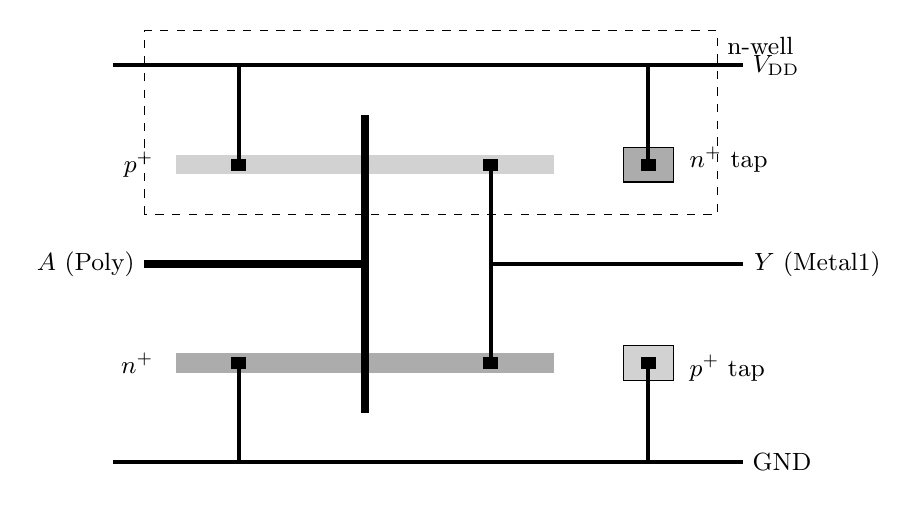
\begin{tikzpicture}[x=0.8cm,y=0.63cm,font=\small]
\draw[dashed] (0.5,5) rectangle (9.6,8.7);
\node[right] at (9.6,8.4) {n-well};
\draw[line width=7pt,gray!35] (1,6)--(7,6);
\draw[line width=7pt,gray!65] (1,2)--(7,2);
\node[left] at (0.8,6) {$p^+$};\node[left] at (0.8,2) {$n^+$};
\draw[line width=3pt] (4,1)--(4,7);
\draw[line width=3pt] (0.5,4)--(4,4);\node[left] at (0.5,4) {$A$ (Poly)};
\draw[line width=1.5pt] (0,8)--(10,8) (0,0)--(10,0);
\node[right] at (10,8) {$V_{\mathrm{DD}}$};\node[right] at (10,0) {GND};
\draw[line width=1.5pt] (2,6)--(2,8) (2,2)--(2,0);
\draw[line width=1.5pt] (6,6)--(6,2);
\draw[line width=1.5pt] (6,4)--(10,4) node[right] {$Y$ (Metal1)};
\draw[fill=gray!65] (8.1,5.65) rectangle (8.9,6.35);
\draw[fill=gray!35] (8.1,1.65) rectangle (8.9,2.35);
\draw[line width=1.5pt] (8.5,6)--(8.5,8) (8.5,2)--(8.5,0);
\foreach \x/\y in {2/6,6/6,2/2,6/2,8.5/6,8.5/2} {
\fill (\x-0.12,\y-0.12) rectangle (\x+0.12,\y+0.12);}
\node[right,align=left] at (9,6.1) {$n^+$ tap};
\node[right,align=left] at (9,1.9) {$p^+$ tap};
\end{tikzpicture}
\end{latin}
\caption{نمای بالای مفهومی \lr{Inverter} بر پایه شکل‌های \secnum{۱.۴۱}
و \secnum{۱.۳۵} کتاب \cite{weste}.
نوار خاکستری بالا \(p^+\)، پایین \(n^+\)، خط عمودی ضخیم وسط \lr{Poly}
و خط‌های نازک سیاه \lr{Metal1} هستند. ابعاد به مقیاس قواعد رسم نشده‌اند؛
این شکل توپولوژی است و ادعای عبور از \lr{DRC} ندارد.}
\label{fig:layout-inverter}
\end{figure}

در نوار پایین، تقاطع \lr{Poly} با \(n^+\) یک \lr{nMOS} می‌سازد؛
سمت چپ از تماس به زمین و سمت راست به خروجی می‌رود.
در نوار بالا یک \lr{pMOS} ساخته می‌شود؛ چپ آن به تغذیه و راست آن به همان خروجی وصل است.
ورودی، نوار \lr{Poly} مشترک است.
تماس‌های جداگانه سمت راست، بدنه‌ها را به ریل مربوط می‌رسانند؛
دو تماس خروجی و دو تماس بدنه یکی نیستند.

برای استخراج شماتیک، ابتدا دو تقاطع ترانزیستوری را بشمارید؛ سپس شبکه‌های فلزی
و تماس‌هایشان را دنبال کنید. نتیجه باید دقیقاً همان دو ترانزیستور با
\lr{Gate} مشترک و \lr{Drain} مشترک باشد.
اگر تماس خروجی یکی حذف شود، دیگر آن اتصال رسانشی در مدل نقشه برقرار نیست؛
اگر تماس ناخواسته روی محل نامناسب اضافه شود، ممکن است شبکه‌های مستقل اتصال کوتاه شوند.

\subsection{اشتراک \lr{Diffusion} و گیت \lr{NAND} سه‌ورودی}
سه \lr{Poly} با ورودی‌های \(A,B,C\) یک نوار \lr{n-diffusion} را قطع می‌کنند.
چهار ناحیه میان دو انتها و سه \lr{Gate} داریم: از سمت خروجی به زمین،
\(Y,x_1,x_2,GND\). کانال‌های میان آن‌ها به‌ترتیب با \(A,B,C\) کنترل می‌شوند.
گره‌های \(x_1,x_2\) داخلی‌اند و برای اتصال سری نیازی به تماس فلزی جدا ندارند؛
ناحیه مشترک، پایانه دو ترانزیستور مجاور را می‌سازد.

همان سه خط \lr{Poly}، نوار \lr{p-diffusion} را نیز قطع می‌کنند.
اگر فقط دو انتهای این نوار را سیم‌کشی کنیم، سه \lr{pMOS} سری خواهیم داشت؛
این برای \lr{NAND} درست نیست. باید چهار ناحیه بالایی را با فلز به‌ترتیب
به \(V_{\mathrm{DD}},Y,V_{\mathrm{DD}},Y\) وصل کنیم.
در نتیجه هر \lr{pMOS} میان همان دو گره تغذیه و خروجی قرار می‌گیرد و موازی است.
شکل \ref{fig:layout-nand-chain} این تمایز را نشان می‌دهد
\cite[شکل \secnum{۱.۴۲}]{weste}.

\begin{figure}[ht]
\centering
\begin{latin}
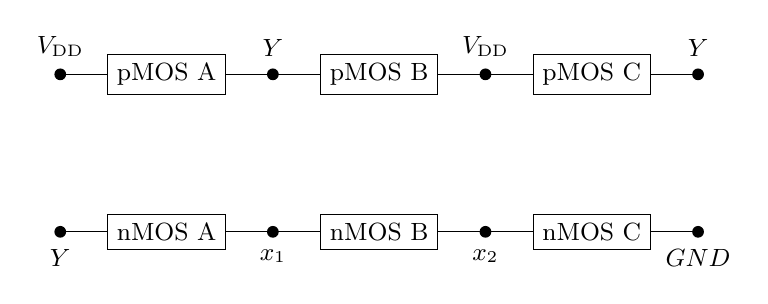
\begin{tikzpicture}[x=1.35cm,y=1cm,font=\small]
\foreach \x/\lab in {0/{V_{\mathrm{DD}}},2/Y,4/{V_{\mathrm{DD}}},6/Y} {
\node[circle,fill,inner sep=1.5pt] at (\x,2) {};
\node[above] at (\x,2.1) {$\lab$};}
\foreach \x/\lab in {1/A,3/B,5/C} {
\draw (\x-1,2)--(\x+1,2) node[midway,draw,fill=white] {pMOS \lab};}
\foreach \x/\lab in {0/Y,2/{x_1},4/{x_2},6/{GND}} {
\node[circle,fill,inner sep=1.5pt] at (\x,0) {};
\node[below] at (\x,-0.1) {$\lab$};}
\foreach \x/\lab in {1/A,3/B,5/C} {
\draw (\x-1,0)--(\x+1,0) node[midway,draw,fill=white] {nMOS \lab};}
\end{tikzpicture}
\end{latin}
\caption{نمای اتصال ناحیه‌های متوالی \lr{Diffusion} در \lr{NAND} سه‌ورودی.
این شکل نمودار اتصال است، نه شماتیک ابعادی: گره‌های هم‌نام بالا با فلز مشترک
می‌شوند؛ دو گره داخلی پایین مستقل‌اند. بلوک‌ها کانال‌های کنترل‌شده‌اند و سیم ثابت نیستند.}
\label{fig:layout-nand-chain}
\end{figure}

شکل \ref{fig:layout-nand-stick} همین اتصال‌ها را در نمای لایه‌ای نشان می‌دهد.
ابتدا فقط نوارهای \lr{Diffusion} و سه خط \lr{Poly} را بخوانید؛
سپس بررسی کنید هر تماس با کدام سیم فلزی به ریل یا خروجی وصل شده است.
\begin{figure}[ht]
\centering
\begin{latin}
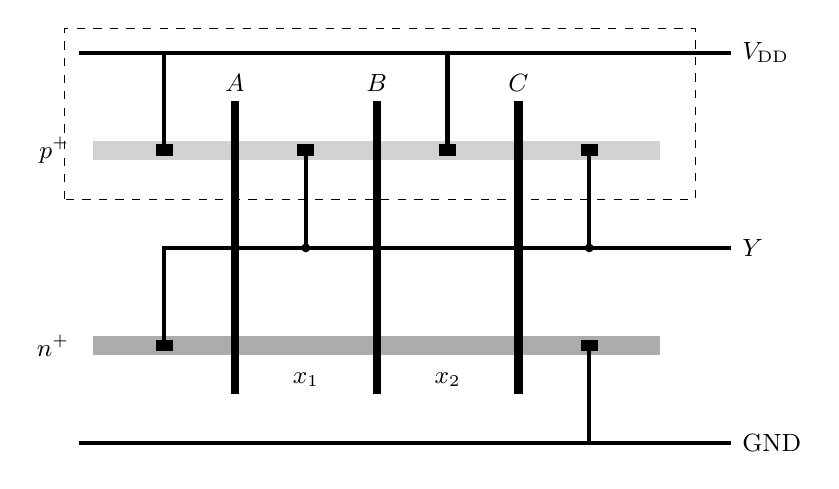
\begin{tikzpicture}[x=0.9cm,y=0.62cm,font=\small]
\draw[dashed] (-0.4,5) rectangle (8.5,8.5);
\draw[line width=7pt,gray!35] (0,6)--(8,6);
\draw[line width=7pt,gray!65] (0,2)--(8,2);
\node[left] at (-0.2,6) {$p^+$};\node[left] at (-0.2,2) {$n^+$};
\foreach \x/\lab in {2/A,4/B,6/C} {
\draw[line width=3pt] (\x,1)--(\x,7);
\node[above] at (\x,7) {$\lab$};}
\draw[line width=1.5pt] (-0.2,8)--(9,8) node[right] {$V_{\mathrm{DD}}$};
\draw[line width=1.5pt] (-0.2,0)--(9,0) node[right] {GND};
\draw[line width=1.5pt] (1,6)--(1,8) (5,6)--(5,8);
\draw[line width=1.5pt] (3,6)--(3,4) (7,6)--(7,4);
\draw[line width=1.5pt] (1,2)--(1,4)--(9,4) node[right] {$Y$};
\draw[line width=1.5pt] (7,2)--(7,0);
\foreach \x/\y in {1/6,3/6,5/6,7/6,1/2,7/2} {
\fill (\x-0.12,\y-0.12) rectangle (\x+0.12,\y+0.12);}
\foreach \x in {3,7} {\fill (\x,4) circle (1.6pt);}
\node at (3,1.3) {$x_1$};\node at (5,1.3) {$x_2$};
\end{tikzpicture}
\end{latin}
\caption{\lr{Stick Diagram} آموزشی \lr{NAND} سه‌ورودی بر پایه شکل‌های
\secnum{۱.۴۲} و \secnum{۱.۴۳} کتاب \cite{weste}.
خط‌های عمودی ضخیم \lr{Poly} و خطوط نازک سیاه \lr{Metal1} هستند؛
تقاطع آن‌ها در مسیر افقی \(Y\) بدون تماس است.
مربع‌ها تماس فلز با \lr{Diffusion} و نقطه‌های گرد اتصال فلز با فلزند.
تماس‌های بدنه برای خلوت ماندن شکل حذف شده‌اند و باید در \lr{Layout} نهایی اضافه شوند؛
اندازه‌های شکل مطابق قواعد رسم نشده‌اند.}
\label{fig:layout-nand-stick}
\end{figure}

در ورودی \((A,B,C)=(1,1,1)\)، سه کانال پایین هدایت دارند و خروجی به زمین می‌رسد؛
هر سه \lr{pMOS} قطع‌اند. اگر مثلاً \(B=0\)، کانال میانی پایین قطع و
\lr{pMOS} مربوط به \(B\) روشن است؛ چون دو سر آن با فلز به خروجی و تغذیه
وصل‌اند، خروجی یک می‌شود. این استدلال برای صفر بودن \(A\) یا \(C\) نیز برقرار است.

اشتراک ناحیه می‌تواند تماس، سیم و مساحت را کم کند؛ هندسه آن بر ظرفیت
\lr{Diffusion} هم اثر می‌گذارد. بااین‌حال، نمی‌توان هر دو ناحیه دلخواه را
ادغام کرد؛ نوع ماده، چاه و شبکه الکتریکی باید سازگار باشند.
یکسان بودن ظاهر خط \lr{Diffusion} به معنی یکسان بودن همه گره‌های آن در حضور
\lr{Gate}های قطع‌کننده مسیر نیست.

\subsection{ریل‌ها، کنارهم‌گذاری سلول و دسترسی پایه}
در سبک کتاب، ریل‌های فلزی بالا و پایین تا مرز سلول ادامه دارند.
فاصله مرزی باید طوری باشد که کنارهم‌گذاری دو سلول نیز قواعد را حفظ کند؛
کتاب در مثال، بیرون‌زدگی \(2\lambda\) ریل در هر طرف را برای تامین فاصله
\(4\lambda\) محتوای دو سلول توضیح می‌دهد.
این عدد به هندسه همان شکل وابسته است، نه قاعده عمومی همه مرزهای سلول
\cite[صفحه چاپی ۲۷]{weste}.

دسترسی به پایه فقط نام‌گذاری آن نیست؛ باید مسیر و فضای اتصال برای سیم‌کشی
سلول‌های دیگر وجود داشته باشد. مثال ساده کتاب اجازه دسترسی \lr{Poly} از بالا
یا پایین را می‌دهد؛ ادامه متن توضیح می‌دهد که دسترسی فلزی و تماس‌های
\lr{Metal2--Metal1--Poly} در سبک‌های دیگر می‌تواند فضای بیشتری لازم داشته باشد.
پس کوچک‌ترین نقشه داخلی، الزاماً بهترین سلول قابل مسیریابی نیست.

\section{\lr{Stick Diagram} و برآورد مساحت}
\label{sec:layout-stick}
\subsection{چه چیزی را حفظ و چه چیزی را حذف می‌کنیم؟}
\lr{Stick Diagram} نمایش سریع توپولوژی لایه‌ها و اتصال‌هاست؛
خط‌ها لازم نیست عرض یا فاصله واقعی داشته باشند.
نوع لایه، محل ترانزیستور و تماس و ترتیب اتصال‌ها حفظ می‌شود؛
اما جزئیات مستطیل‌ها و اندازه‌گذاری نهایی به \lr{Layout} واگذار می‌شود
\cite[بخش \secnum{۱.۵.۵}]{weste}.
بنابراین شکل \ref{fig:layout-inverter} از نظر نقش آموزشی به یک \lr{Stick Diagram}
نزدیک است؛ مرز تماس‌ها و چاه فقط برای فهم بهتر اضافه شده‌اند.
صرف کشیدن یک طرح باریک، مساحت کمتر قابل ساخت را اثبات نمی‌کند.

\subsection{از \lr{Routing Track} به ابعاد تقریبی}
یک \lr{Routing Track} فضایی برای یک سیم و فاصله لازم تا سیم مجاور است.
برای عرض فلز \(4\lambda\) و فاصله آزاد \(4\lambda\)،
\lr{Track Pitch} برابر \(8\lambda\) می‌شود.
اگر \(N_x\) و \(N_y\) تعداد بازه‌های ترک در دو جهت باشند، تخمین اولیه این است:
\begin{equation}\label{eq:layout-area}
W_{\mathrm{cell}}\approx8\lambda N_x,\qquad
H_{\mathrm{cell}}\approx8\lambda N_y,\qquad
A_{\mathrm{cell}}\approx64N_xN_y\lambda^2.
\end{equation}
در رابطه سوم، دو طول را ضرب کردیم؛ پس واحد مساحت \(\lambda^2\) است، نه
\(\lambda\). این تقریب به سبک و قواعد همان مدل متکی است.
شمارش \lr{Track} به معنی شمردن تعداد ترانزیستور یا صرفاً تعداد خط‌های مرئی نیست؛
فضاهای لازم و حاشیه‌ها هم سهم دارند.

مرز چاه باید از \lr{pMOS} به اندازه \(6\lambda\) فاصله پوشش داشته باشد
و از \lr{nMOS} نیز \(6\lambda\) دور باشد. بنابراین در این مدل،
میان دو ناحیه ترانزیستوری حداقل فضای \(12\lambda\) لازم می‌شود.
کتاب اثر این فاصله را با اختصاص یک \lr{Track} اضافی میان دو ردیف لحاظ می‌کند؛
حتی اگر آن ترک واقعاً سیمی نداشته باشد
\cite[شکل‌های \secnum{۱.۴۴} و \secnum{۱.۴۵}]{weste}.
نباید \(12\lambda\) را با فاصله آزاد معمول فلز \(4\lambda\) یکی گرفت.

\subsection{مثال کتاب: مساحت \lr{NAND} سه‌ورودی}
در شکل \secnum{۱.۴۶} کتاب، چهار ترک در جهت عرض و پنج ترک در جهت ارتفاع
شمارش شده‌اند. بنابراین:
\begin{equation*}
W_{\mathrm{cell}}\approx32\lambda,\qquad
H_{\mathrm{cell}}\approx40\lambda,\qquad
A_{\mathrm{cell}}\approx1280\lambda^2.
\end{equation*}
کتاب ارتفاع بدنه سلول را \(36\lambda\) و ارتفاع با فضای اضافی
\(4\lambda\) مجاور را \(40\lambda\) معرفی می‌کند؛
اختلاف این دو عدد ناشی از تعریف مرز شمارش مساحت است
\cite[صفحات چاپی ۲۷ تا ۲۹]{weste}.
هنگام مقایسه دو مساحت باید معلوم باشد فاصله بین سلول‌ها نیز شمرده شده است یا نه.

با انتخاب آموزشی \(\lambda=\qty{0.3}{\micro\metre}\)، ابعاد و مساحت می‌شوند:
\begin{align*}
W_{\mathrm{cell}}&\approx\qty{9.6}{\micro\metre},&
H_{\mathrm{cell}}&\approx\qty{12}{\micro\metre},\\
A_{\mathrm{cell}}&\approx1280(0.3)^2\,\unit{\square\micro\metre}
=\qty{115.2}{\square\micro\metre}.
\end{align*}
ضریب \(0.3\) باید به توان دو برسد؛ زیرا تبدیل واحد مساحت از ضرب دو طول می‌آید.
این عدد، برآورد هندسی با ورودی‌های فرض‌شده است و گزارش اندازه‌گیری یک تراشه نیست.

\subsection{مثال کتاب: گیت \lr{OAI31}}
تابع مثال \secnum{۱.۳} کتاب،
\(Y=\overline{(A+B+C)D}\) است؛ مکمل روی کل عبارت قرار دارد.
پایین، گروه موازی \(A,B,C\) با \(D\) سری و بالا، گروه سری \(A,B,C\)
با \(D\) موازی می‌شود.
برای شکل \secnum{۱.۴۷}، کتاب پنج و شش ترک را در دو جهت گزارش می‌کند،
پس ابعاد تخمینی \(40\lambda\times48\lambda\) و مساحت
\(1920\lambda^2\) است \cite[صفحه چاپی ۲۹]{weste}.
این تخمین برای همان ترتیب و مسیرهای شکل است؛ بهینه بودن آن برای هر فرایند اثبات نشده است.

با مقیاس مثال قبلی، ابعاد \(\qty{12}{\micro\metre}\) و
\(\qty{14.4}{\micro\metre}\) و مساحت
\(\qty{172.8}{\square\micro\metre}\) می‌شود.
نسبت مساحت به \lr{NAND} قبلی برابر \(1920/1280=1.5\) است؛
این نسبت برای دو برآورد با قواعد و مرز یکسان معتبر است.

\subsection{چرا این برآورد محدود است؟}
اگر عرض ترانزیستور از \(4\lambda\) بیشتر شود، فضای اضافه آن باید لحاظ شود.
تعداد و محل تماس‌ها، دسترسی پایه، لایه فلزی، مرز چاه و سیم‌کشی نیز
می‌توانند تعداد ترک لازم را تغییر دهند.
پس رابطه \eqref{eq:layout-area} نقشه راه اولیه است، نه جانشین طراحی دقیق
و کنترل قواعد کامل. کتاب نیز برای سلول‌های حساس، ساخت آزمایشی \lr{Layout}
را لازم می‌داند \cite[ابتدای صفحه چاپی ۲۹]{weste}.

\section{تمرین‌های جمع‌بندی و پاسخ تشریحی}
\subsection{پرسش‌ها}
\begin{enumerate}
\item اگر یک خط فلز از روی \lr{Poly} عبور کند و تماس نداشته باشد، آیا دو شبکه متصل‌اند؟
\item چرا در نوار \lr{p-diffusion} گیت \lr{NAND}، سیم‌کشی همه گره‌ها به یک فلز مشترک غلط است؟
\item برای \(\lambda=\qty{0.1}{\micro\metre}\)، عرض \(4\lambda\)،
تماس \(2\lambda\) و مساحت \(1280\lambda^2\) را به واحد فیزیکی تبدیل کنید.
\item سه خط \lr{Metal1} به عرض \(4\lambda\)، با دو فاصله آزاد
\(4\lambda\)، مجموعاً چه پهنایی اشغال می‌کنند؟ فاصله مرکز خط اول تا سوم چقدر است؟
\item اگر در همان مدل تخمین، مقیاس \(\lambda\) نصف شود، طول‌ها و مساحت چه تغییری می‌کنند؟
آیا این نتیجه امکان انتقال مستقیم نقشه به هر فرایند دیگری را ثابت می‌کند؟
\end{enumerate}

\subsection{پاسخ‌ها و کنترل نتیجه}
\begin{enumerate}
\item در مدل لایه‌های عایق‌شده خیر؛ برای اتصال \lr{Metal1} به \lr{Poly}
تماس مناسب لازم است. در مقابل، عبور \lr{Poly} از \lr{Active} نقش ترانزیستوری دارد.
\item همه گره‌های میان کانال‌ها نباید یک شبکه باشند؛ با اتصال همگی به یک فلز،
دو ریل یا پایانه‌های لازم کوتاه می‌شوند و نقش ترانزیستورها از بین می‌رود.
در مثال، گره‌های متوالی باید به‌تناوب تغذیه و خروجی باشند.
\item عرض \(\qty{0.4}{\micro\metre}\)، ضلع تماس
\(\qty{0.2}{\micro\metre}\) و مساحت
\(1280(0.1)^2=\qty{12.8}{\square\micro\metre}\) است.
\item پهنای لبه بیرونی تا لبه بیرونی برابر
\((3\times4+2\times4)\lambda=20\lambda\) است.
فاصله مرکز اول تا سوم دو \lr{Pitch}، یعنی \(16\lambda\) است؛
این دو اندازه یکسان نیستند. برای \(n\) خط هم‌اندازه، پهنای فیزیکی
\(nw+(n-1)s\) و فاصله دو مرکز انتهایی \((n-1)(w+s)\) خواهد بود.
\item در مدل تشابه هندسی، هر طول نصف و مساحت یک‌چهارم می‌شود.
اما قواعد واقعی ممکن است یکسان مقیاس نشوند؛ پس قابلیت ساخت در فرایند دیگر
از این محاسبه نتیجه نمی‌شود.
\end{enumerate}

\subsection{روش بازبینی یک طرح تازه}
ابتدا تعداد تقاطع‌های \lr{Poly/Active} را با تعداد ترانزیستورهای شماتیک مقایسه کنید.
سپس هر ناحیه \lr{Diffusion}، فلز و تماس را به یک شبکه نام‌گذاری‌شده نسبت دهید.
نوع ترانزیستور و اتصال بدنه را کنترل کنید؛ در پایان ابعاد، فاصله‌ها و دسترسی پایه‌ها را بررسی کنید.
این ترتیب، خطای اتصال را از خطای هندسی جدا می‌کند.

در ابزارهای طراحی، \lr{DRC} قواعد هندسی و \lr{LVS} تطبیق مدار استخراج‌شده با
شماتیک را بررسی می‌کنند؛ عبور از یکی به معنی عبور از دیگری نیست.
در این جزوه کنترل‌های آموزشی محاسبه و توپولوژی انجام می‌شوند؛
تایید صنعتی به فایل‌های فرایند و ابزارهای مربوط نیاز دارد.
با این پایه، می‌توان در ادامه فصل از طراحی یک سلول به سازمان‌دهی یک مدار بزرگ‌تر رسید.
